\chapter{肌肉结构和动力学} \label{chap:chap5}


如果你想理解功能,那就研究结构。

\begin{flushright}
	——弗朗西斯$\cdot$克里克
\end{flushright}


\begin{figure}[!htb]
	\centering
	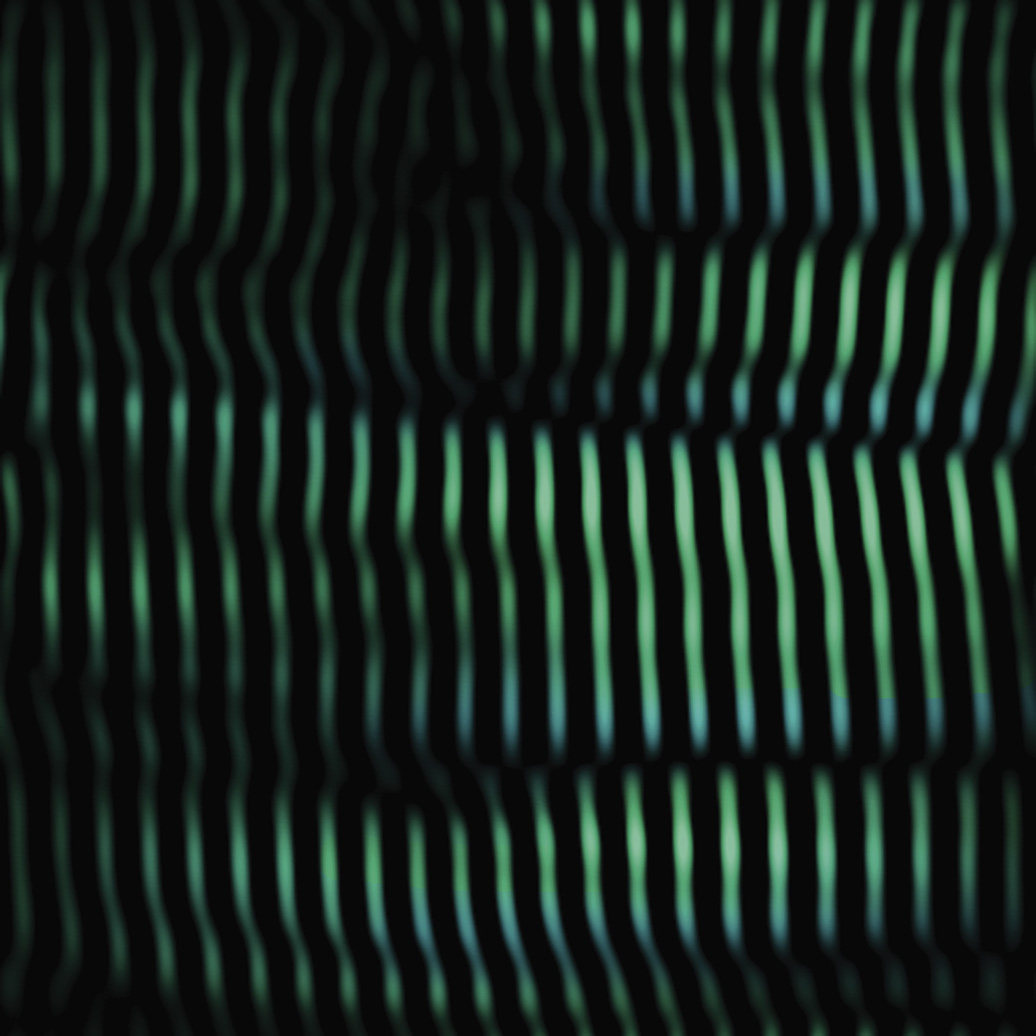
\includegraphics[width=1.0\linewidth]{chap4/4_0}
	% 加星号(*)表示不加编号
	\caption*{ \label{fig:5_0}}
\end{figure}


为了理解人类和动物的运动,研究人员开展了各种各样的实验。
生物力学家通过测量数千人的关节运动、地面反作用力和肌电信号来研究全身运动。
生理学家研究了单个肌肉,以表征肌肉激活和力量产生的动态。
肌肉驱动模拟使我们能够将这两个领域联系起来,将全身运动的生物力学测量与针对单个肌肉进行的实验相结合。
我们将在第~\ref{chap:chap10}~至~\ref{chap:chap12}~章中看到,肌肉驱动模拟可以深入了解肌肉在产生运动中的作用,并提供一些在人体运动时几乎无法测量的重要量的估计值,例如肌肉产生的力量和它消耗的能量。


肌肉动力学建模对于创建肌肉驱动的运动模拟至关重要。
然而,一刀切的模型并不适用,因为每块肌肉都有其独特的结构来适应其独特的功能。
例如,一些肌肉负责手指的精细运动控制,而另一些肌肉则在运动过程中支撑身体重量(图~\ref{fig:5_1})。
所有骨骼肌都具有肌节的层级排列,但肌肉在几个重要方面存在差异。
这些差异包括它们的大小和结构,以及肌肉纤维的几何排列。
因此,肌肉的计算模型必须捕捉所有肌肉共同的肌肉力量产生特征,同时还要能够表征每块肌肉的独特特征。


\begin{figure}[!htb]
	\centering
	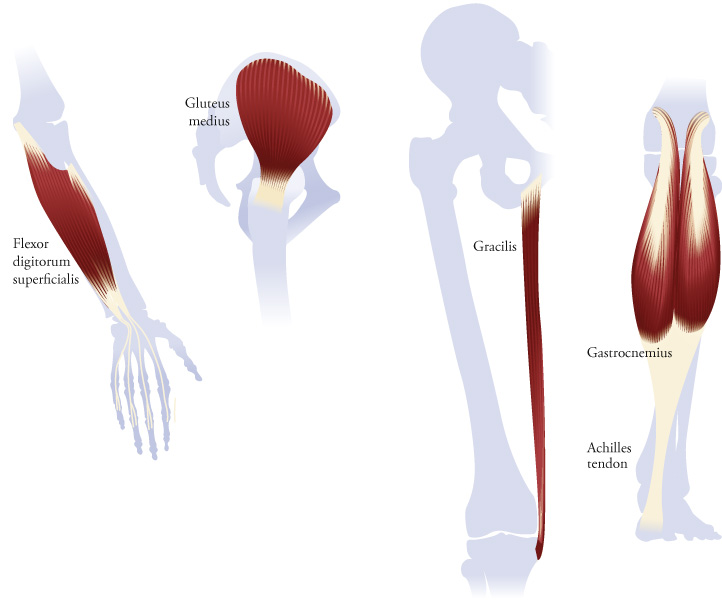
\includegraphics[width=1.0\linewidth]{chap5/5_1}
	\caption{全身肌肉的结构和功能各不相同。
		浅屈指肌(最左侧)通过四条肌腱控制手指屈曲;
		宽阔的臀中肌和纤细的股薄肌产生髋关节外展和内收力矩;
		腓肠肌(最右侧)通过较长的跟腱止于跟骨。 \label{fig:5_1}}
\end{figure}


在本章中,我们将了解如何创建一个通用的肌肉力量产生模型,以及如何对其进行定制以代表身体中的几乎任何肌肉。
我们将要描述的肌肉模型属于以 A. V. Hill 命名的一类模型,除了我们在第~\ref{chap:chap4}~章中看到的“推我拉你”实验之外,他还进行了许多肌肉的基础研究。
我的博士生导师 Felix Zajac 改进了 Hill 型模型,并将其带入了现代计算机模拟时代\cite{zajac1989muscle}。
具体来说,Zajac 开发了一个仅包含四条通用曲线和五个肌肉特定参数的模型,所有这些参数都可以从实验数据中得出并用于调整模型。
Zajac 模型的简单性对于涉及数十块肌肉的动态模拟至关重要,但它足够详细,可以表示不同大小、强度和结构的肌肉的动态。


图~\ref{fig:4_18}~总结了所有肌肉共同的肌肉力量产生特征。
这些特征包括 3 条曲线,描述肌肉长度与其产生的力之间的非线性关系:主动力-长度曲线、被动力-长度曲线和力-速度曲线。
由于肌肉通过肌腱附着在骨骼上,我们还必须考虑这种结缔组织的特性,我们用肌腱的力-长度曲线来描述它。
我们使用 5 个参数缩放这些通用曲线以表示特定的肌肉:
(1)最佳肌纤维长度 $l_o^M$;
(2)最佳纤维长度下的肌纤维羽状角 $\phi_o$ ;
(3)最大等长肌肉力量,$F_o^M$;
(4)最大肌肉收缩速度 $v_\text{max}^M$;
和(5)肌腱松弛长度,$l_s^T$。
本章首先介绍这 5 个特定于肌肉的参数。
我们将了解每个参数如何影响肌肉力量,并将其纳入肌肉-肌腱动力学模型中。


\section{最佳肌纤维长度$l_o^M$}

正如我们在第~\ref{chap:chap4}~章中看到的,肌节能够产生的主动力取决于其长度(图~\ref{fig:4_6})。
肌节能够产生最大等长收缩力的长度称为其最佳长度。
由于肌纤维由多个($n$)个首尾相连的肌节组成,因此肌纤维也存在一个最佳长度($l_o^M$),当其每个组成肌节都达到其最佳长度($l_o^S$)时,肌纤维便会达到该最佳长度:
%
\begin{equation}
	l_o^M = n l_o^S \label{eq:5_1}
\end{equation}

公式~\ref{eq:5_1}~假设肌纤维上串联的所有肌节长度相同。
肌肉在运动过程中会伸长和缩短,这会影响肌节粗肌丝和细肌丝相互滑动时产生的主动力。
最佳长度较长的肌纤维(即串联肌节较多)具有更宽的主动力-长度曲线,并且可以在更宽的长度范围内产生其最大主动力的很大一部分(图~\ref{fig:5_2},顶部)。
增加肌纤维的最佳长度也会增加其最大缩短速度():

\begin{figure}[!htb]
	\centering
	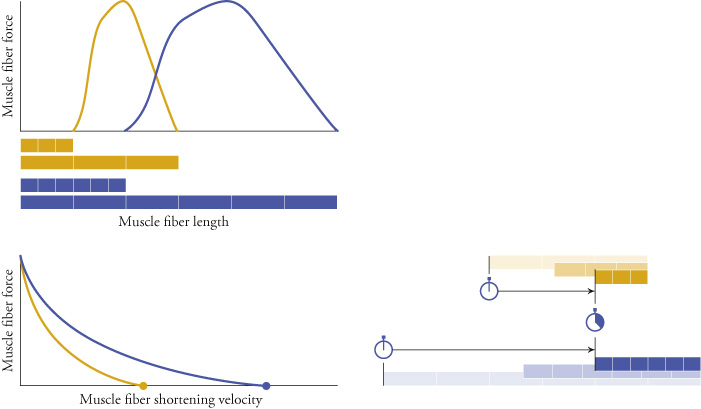
\includegraphics[width=1.0\linewidth]{chap5/5_2}
	\caption{最佳肌纤维长度较长的肌肉,其主动力-长度曲线(上图)更宽,最大缩短速度也更高(下图)。
		请注意,长肌纤维(蓝色)的示意图中,肌节数量是短肌纤维(橙色)的两倍,因此长肌纤维在给定时间内可以缩短 2 倍的距离(右下图)。 \label{fig:5_2}}
\end{figure}

\begin{equation}
	v_{\text{max}}^M = n v_{\text{max}}^S \label{eq:5_2}
\end{equation}
%
其中,$v_\text{max}^S$表示肌节的最大缩短速度。
因此,随着肌肉最佳纤维长度的增加,力-速度曲线也会变宽(图~\ref{fig:5_2},底部)。


生物肌肉由长度不同的肌束构成,肌束本身包含长度也不同的纤维,这些纤维甚至可能终止于肌束内。
然而,在我们的模型中,我们假设肌肉中的所有纤维长度相同——许多(但并非所有)肌肉-肌腱动力学模型都做出了这一假设。
我们进一步假设所有纤维都是直的、平行的且共面的。
因此,为了表征肌肉的力-长度和力-速度特性,我们只是放大了肌纤维的相应特性,而这些特性仅仅是肌节相同特性的放大版本。



\section{最佳纤维长度下的肌纤维羽状角$\phi_o$}

肌肉通常通过肌腱附着于骨骼。
在平行纤维肌腱中,例如缝匠肌,其纤维沿着肌腱方向排列(图~\ref{fig:5_3})。
在大多数其他肌肉中,例如股直肌,其纤维与肌腱呈锐角排列;我们称这些肌肉为羽状肌。
“羽状肌”一词源于拉丁语,意为“羽毛状”,而羽状肌的结构确实让人联想到鸟类的羽毛。

\begin{figure}[!htb]
	\centering
	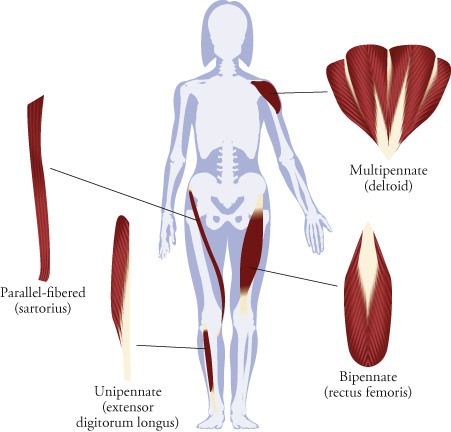
\includegraphics[width=0.8\linewidth]{chap5/5_3}
	\caption{具有不同结构的肌肉的例子:
		平行纤维肌肉、单羽状肌肉、双羽状肌肉和多羽状肌肉。 \label{fig:5_3}}
\end{figure}

如果所有肌纤维都附着在肌腱的一侧,我们称该肌肉为单羽状肌;如果肌纤维附着在肌腱的两侧,则称该肌肉为双羽状肌。
在多羽状肌中,肌腱分支和肌纤维结构可能很复杂。
因此,我们假设给定肌肉中的所有纤维都以相同的角度(称为羽状角 ($\phi$))附着于肌腱,并采用图~\ref{fig:5_4}~所示的肌肉-肌腱几何模型。
由此,我们得到肌纤维中的力 ($F^M$) 和肌腱中的力 ($F^T$) 之间的以下关系:

\begin{figure}[!htb]
	\centering
	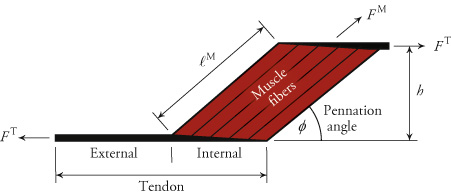
\includegraphics[width=0.75\linewidth]{chap5/5_4}
	\caption{肌纤维和肌腱的简化几何表示。
		肌纤维被假设为直的、平行的、共面的、等长的,并以相同的羽状角 ($\phi$) 附着于肌腱。
			当肌纤维缩短或伸长,羽状角增大或减小时,平行四边形的高度 $h$(以及面积)保持不变\cite{zajac1989muscle}。 \label{fig:5_4}}
\end{figure}

\begin{equation}
	F^T = F^M cos(\phi) 
	\label{eq:5_3}
\end{equation}

现在,参考图~\ref{fig:5_4},我们可以解释生物肌肉如何在纤维长度发生变化的情况下保持体积恒定。
随着图中纤维的缩短,想象一下它们以这样的方式缩短,使得图~\ref{fig:5_4}中的平行四边形保持相同的高度 $h$。
平行四边形的顶部将保持不变,但底部将被向右拉,平行四边形将变得更接近矩形。
然而,只要高度保持不变,面积也将保持不变,这符合平行四边形面积等于其底边和高乘积的几何规则。
我们以二维方式绘制了该图,但三维运动类似,并确保肌肉的体积不变。
简而言之,羽状肌不是通过膨胀来维持体积,而是通过剪切来维持体积。


在上述过程中,羽状角不断增大,从纤维传递到肌腱的力不断减小,直到纤维与肌腱垂直,图中的肌肉呈矩形(即$\phi$ = 90度)。
我们使用参数$\phi_o$表示肌纤维达到最佳长度时的羽状角(即$l^M = l_o^M$)。
我们所描述的固定高度近似法可能会对收缩时明显隆起的肌肉引入误差,但它为研究肌肉结构的功能含义提供了一个简单的几何模型。


除了公式~\ref{eq:5_3}~中表达的关系外,羽状肌在决定肌肉的产力能力方面也起着至关重要的作用。
一般来说,羽状肌角度越大,在给定体积内能够容纳的肌肉纤维越多。
想象一下在矩形房间铺设硬木地板的类似情况:可以使用相对较少的长木板来延伸房间的长度,或者使用大量较短的木板以对角线方向铺设。
同样,与相同体积的平行纤维肌肉相比,羽状肌的纤维更短,因此主动力-长度曲线和力-速度曲线更窄(图~\ref{fig:5_2})。
当然,羽状肌也包含更多的纤维,其后果将在下一节探讨。



\section{最大等长肌肉力量$F_o^M$}

我们 5 个肌肉参数系列中的第三个参数相对容易理解,但测量起来却不那么容易。
这就是最大等长肌肉力。
它被定义为肌肉在最大程度激活并保持最佳纤维长度时产生的力量。


对于活体人体来说,最大等长肌力很难测量,因为我们无法将一块肌肉与其他肌肉分离,并只对该肌肉施加阻力。
因此,我们使用一个称为生理横截面积(PCSA;图~\ref{fig:5_5})的指标。
这是肌肉垂直于纤维方向的横截面积。
需要注意的是,在羽状肌中,该横截面积与肌肉的纵轴倾斜。
最大等长肌力可以通过以下方式估算:

\begin{figure}[!htb]
	\centering
	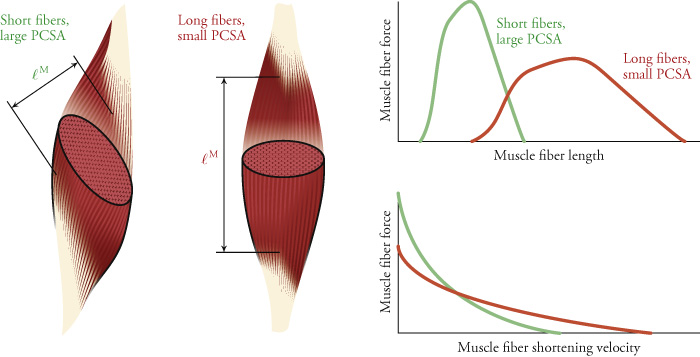
\includegraphics[width=1.0\linewidth]{chap5/5_5}
	\caption{左图所示的肌肉体积相同,但PCSA(主成分分析面积)、最佳纤维长度和羽状角不同。
		羽状肌越多,产生的主动力越大,但纤维越短;
		因此,其主动力-长度曲线和动力-速度曲线更高,但更窄\cite{lieber2002skeletal}。 \label{fig:5_5}}
\end{figure}

\begin{equation}
	F_o^M = \text{PCSA} \sigma_o^M
	\label{eq:5_4}
\end{equation}
%
其中 $\sigma_o^M$ 是肌肉的比张力(也称为峰值等长应力),即单位面积可产生的最大肌肉力。
在构建健康肌肉模型时,该参数的典型值为 $\sigma_o^M = 0.3 \; \text{MPa}$ 。


在上一节中,我们注意到,羽状肌的纤维比相同体积的平行纤维肌更短,但数量也更多。
因此,尽管羽状肌的力-长度和力-速度曲线较窄,但这些曲线也会更高,因为羽状肌的PCSA(以及因此产生的最大等长力)更大(图~\ref{fig:5_5})。


肌肉纤维的长度和收缩速度不仅仅受其几何形状的影响,我们将在接下来的两节中看到这一点。
尽管如此,我们已经可以观察到肌肉的结构如何影响其所能执行的功能范围:
在其他条件相同的情况下,羽状肌能够比相同体积的平行纤维肌产生更大的力量,但其长度范围较小,收缩速度也较低。



\section{最大肌肉收缩速度$v_\text{max}^M$}

到目前为止,我们已经介绍了 3 个与肌肉纤维几何排列相关的变量。
为了确定肌肉的最大收缩速度,我们现在引入一个概念:
肌肉纤维有两种类型:快肌纤维和慢肌纤维。
在单次收缩实验中(图~\ref{fig:4_12}),快肌纤维具有更快的上升时间和松弛时间,并且最大收缩速度也更高——大约为每秒 10 个最佳纤维长度 (10 $l_o^M / s$),而慢肌纤维约为 3 $l_o^M / s$ 个。
哺乳动物的肌肉同时包含这 2 种类型的纤维,但快肌纤维与慢肌纤维的比例会因肌肉的功能而异。
例如,腓肠肌含有大量的快肌纤维,这些纤维在需要快速产生巨大力量的活动(例如短跑)中被募集。
邻近的比目鱼肌主要由慢肌纤维组成,这些慢肌纤维非常适合在长时间站立时产生力量,因为慢肌纤维耐疲劳。


肌纤维不仅以其收缩速度区分,还以其产生ATP的方式区分。
有氧(即利用氧气)产生ATP的肌纤维比无氧(即无氧)产生ATP的肌纤维更耐疲劳。
慢肌纤维往往耐疲劳,而快肌纤维则易疲劳。
人类和其他一些动物拥有第三种肌纤维类型,因此我们通常将肌纤维分为I型(慢速,耐疲劳)、IIA型(快速,中度易疲劳)或IIB型(极快,高度易疲劳)。
通过强化训练可以增加快速且仅中度易疲劳的肌纤维比例。


回想一下第~\ref{chap:chap4}~章,运动单位大小各异,中枢神经系统会按照亨尼曼大小原则(图~\ref{fig:4_13})从小到大依次募集运动单位。
除了大小不同之外,运动单位所含纤维的类型也有所不同,同一运动单位中的所有纤维都属于同一类型。
最小的运动单位通常由 I 型纤维组成,最先被募集,其次是由 IIA 型纤维组成的稍大的运动单位。
最大的运动单位包含 IIB 型纤维,通常最后被募集。
因此,在低激活度下(例如在安静站立时可能观察到),主要募集的是慢肌、抗疲劳的运动单位。
因此,在低激活度下,肌肉的最大收缩速度可能会降低;
然而,在肌肉-肌腱动力学模型中,通常假设其为常数 10 $l_o^M/s$。


粗略地说,家禽和鱼类的可疲劳肌纤维和抗疲劳肌纤维是分开的(图~\ref{fig:5_6})。
相反,哺乳动物的肌肉中可疲劳肌纤维和抗疲劳肌纤维是交替分布的。
这就是为什么鸡肉菜肴可以用白肉或黑肉来制作,而牛肉菜肴却不能。
颜色差异的原因是深色肌肉(或肉)富含一种叫做肌红蛋白的蛋白质,这种蛋白质在肌肉中储存氧气,使肌肉颜色变深,使其更耐疲劳。
鸡腿的深色肉由用于长时间站立和奔跑的腿部肌肉(抗疲劳、慢肌纤维)组成。
白色的胸肉由仅用于短时间飞行的肌肉(可疲劳、快肌纤维)组成。
在人类中,单个肌纤维要么是“深色”的,要么是“白色”,但这两种纤维类型都散布在每块肌肉中。


\begin{figure}[!htb]
	\centering
	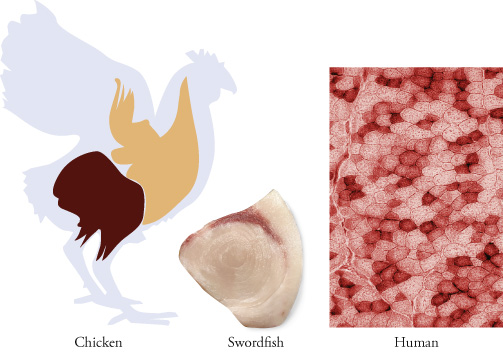
\includegraphics[width=0.8\linewidth]{chap5/5_6}
	\caption{鸡肉和鱼类的某些肌肉主要由抗疲劳的慢肌纤维(深色肉)组成,而另一些肌肉则由易疲劳的快肌纤维(白肉)组成。
		在人类和其他哺乳动物中,各种类型的纤维散布在每块肌肉中。
		人体纤维染色图像显示了不同的纤维类型,由 Richard Lieber 提供。 \label{fig:5_6}}
\end{figure}


\section{肌腱松弛长度 $l_s^T$}

到目前为止,我们讨论的所有参数都与肌腱无关。
在我们的希尔模型中,我们将肌腱描述为非线性弹簧。
本节介绍 5 个参数中的第五个参数,称为肌腱松弛长度,以及四个通用无量纲曲线中的第四个参数,称为肌腱力-长度曲线。
我们根据应力和应变之间的实验测量结果推导出力-长度曲线(图~\ref{fig:5_7})。


\begin{figure}[!htb]
	\centering
	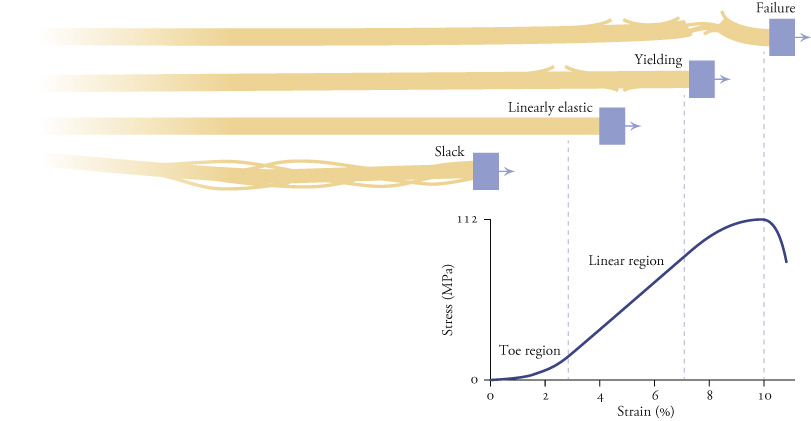
\includegraphics[width=0.8\linewidth]{chap5/5_7}
	\caption{在该图中,横轴表示肌腱的应变,用其长度相对于静止且未受力时的长度的百分比表示。
		静止长度即为松弛长度,用 $l_s^T$ 表示。
		任意给定时刻肌腱的应变 ($\epsilon^T$) 定义如下: \label{fig:5_7}}
\end{figure}

\begin{equation}
	\epsilon^T = \frac{l^T - l_s^T}{l_s^T} 
	\label{eq:5_5}
\end{equation}
% 
其中 $l^T$ 是肌腱的当前长度,$l_s^T$是其松弛长度。


图~\ref{fig:5_7}~中的纵轴表示肌腱单位横截面积产生的力,称为应力。
在线性弹簧中,应力与应变的关系图是一条直线,其斜率表示弹簧的刚度。
由于肌腱充当非线性弹簧,因此应力-应变曲线不是直线,并且它具有三个具有不同刚度特征的区域。
在脚趾区域,当肌腱拉伸约 0\% 到 3\% 时,它会更加柔顺(“有弹性”),随着肌腱的伸长和其组成胶原纤维的展开,其刚度逐渐增加。
在应力-应变曲线的线性区域,当肌腱拉伸约 3\% 到 7\% 时,肌腱具有恒定的刚度;
在此区域,它的行为类似于线性弹簧。
最后,超过 10\% 的应变,肌腱开始出现机械故障,并且存在很高的受伤风险。
我们通常假设内部肌腱(腱膜)和外部肌腱具有相同的材料特性和应变。
有实验证据支持上面给出的应变值,但有人认为肌腱在断裂前可以承受高达 15\% 的更高应变值。


肌腱会影响其所附着肌肉的长度,从而影响其产力能力(图~\ref{fig:5_8})。
如果肌腱的松弛长度相对于肌纤维的长度较短,则肌腱的拉伸几乎不会产生影响:即使这样的肌腱承受很大的应变,其绝对长度变化(以及肌纤维缩短的量)也只是肌纤维最佳长度的一小部分。
相反,如果肌腱的松弛长度相对于肌纤维的最佳长度较长,则肌肉产力时肌腱会大幅拉伸,导致肌纤维明显缩短,并改变产生的主动力。
图~\ref{fig:5_9}~显示,较长的肌腱还可以增加肌肉-肌腱单元产力的长度范围。
通过这两种方式,肌腱都会显著影响肌肉功能。
当然,当肌腱损伤导致肌肉几乎无法使用时,肌腱的作用尤为明显。
正如我们将在第~\ref{chap:chap12}~章中看到的,肌腱在跑步过程中伸展和回缩时也在能量的储存和释放中发挥着重要作用。


\begin{figure}[!htb]
	\centering
	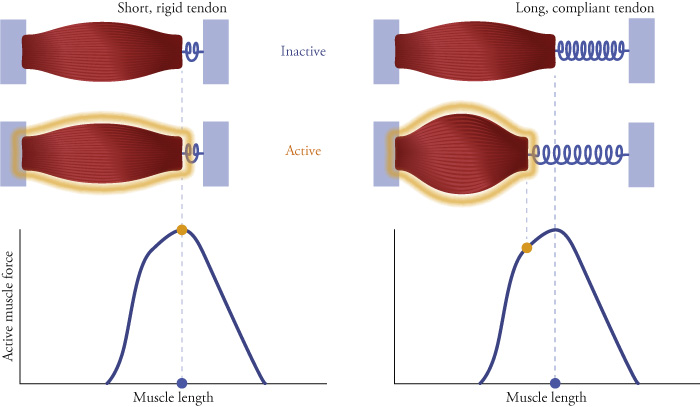
\includegraphics[width=1.0\linewidth]{chap5/5_8}
	\caption{肌腱的柔顺性会影响肌肉力量的产生。
		在图示的两种情况下,平行纤维肌肉在非活动状态时处于最佳长度(上)。
		如果肌腱相对较短且僵硬(左),则肌肉活动时肌纤维的长度变化可以忽略不计。
		如果肌腱较长且柔顺性良好(右),则肌肉活动时肌腱会拉伸,从而缩短肌纤维并减少产生的力量。 \label{fig:5_8}}
\end{figure}


\begin{figure}[!htb]
	\centering
	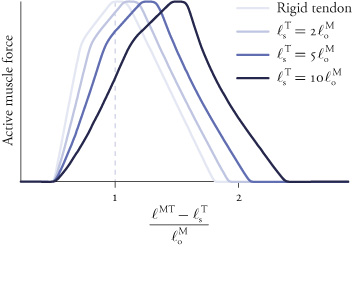
\includegraphics[width=0.6\linewidth]{chap5/5_9}
	\caption{肌腱柔顺性对主动力-长度曲线的影响。
		增加肌腱相对于最佳肌纤维长度的松弛长度(即增加肌腱柔顺性),可以扩大肌肉-肌腱执行器产生主动力的长度范围。 \label{fig:5_9}}
\end{figure}


\section{测量肌肉特定参数}

总而言之,我们定义了五个肌肉特异性参数,列于表~\ref{tab:5_1},这些参数捕捉了身体肌肉之间的大部分变异性。
我们在表 5.2 中列出了下肢主要肌肉的这些参数值。
为方便起见,我们通常将力、速度、肌肉长度和肌腱长度分别除以 、 、 和 来进行归一化,并使用波浪号表示归一化后的量(例如 )。


\begin{table}[htbp]
	\caption{Hill 型模型使用的 5 个肌肉特定参数} \label{tab:5_1} \centering
	\begin{tabular}{ccc} % l水平左居中,c水平居中
		\toprule
		肌肉特异性参数 & 符号 & 典型单位  \\
		\midrule
		最佳纤维长度下的羽状角 & $\phi_o$ &  度 \\
		\midrule
		最大等长力量 & $F_o^M$ &  牛顿 \\
		\midrule
		最大收缩速度 & $v_\text{max}^M$ &  $l_o^M / s$ \\
		\midrule
		肌腱松弛长度 & $l_s^T$ &  厘米 \\
		\bottomrule
	\end{tabular}
\end{table}


\begin{table}[htbp]
	\caption{下肢主要肌肉的肌肉特异性参数值*} \label{tab:5_2} \centering
	\begin{tabular}{ccccc} % l水平左居中,c水平居中
		\toprule
		肌肉 & 最大等长力(牛) & 最佳纤维长度(厘米)& 肌腱松弛长度(厘米) &  羽状角(度) \\
		\midrule
		短收肌 & 626 &  10.3 & 3.5 & 7 \\
		\midrule
		长收肌 & 917 &  10.8 & 13.2 & 8 \\
		\midrule
		大收肌 &  &   &  &  \\
		\midrule
		末梢 & 597 &  17.7 & 8.7 & 11 \\
		\midrule
		坐骨 & 597 &  15.6 & 21.6 & 10 \\
		\midrule
		腰部 & 597 &  13.8 & 4.7 & 12 \\
		\midrule
		近端 & 597 &  10.6 & 4.0 & 18 \\
		\midrule
		股二头肌长头 & 1313 &  9.8 & 32.5 & 10 \\
		\midrule
		股二头肌短头 & 557 &  11.0 & 10.6 & 15 \\
		\midrule
		伸趾长肌 & 603 &  6.9 & 36.9 & 13 \\
		\midrule
		拇长伸肌 & 286 &  7.5 & 32.7 & 11 \\
		\midrule
		屈趾长肌 & 423 &  4.5 & 37.9 & 13 \\
		\midrule
		拇长屈肌 & 908 &  5.3 & 35.4 & 15 \\
		\midrule
		腓肠肌外侧头 & 1575 &  5.9 & 37.6 & 12 \\
		\midrule
		腓肠肌内侧头 & 3116 &  5.1 & 39.9 & 10 \\
		\midrule
		臀大肌 &  &   &  &  \\
		\midrule
		上 & 984 &  14.7 & 4.9 & 20 \\
		\midrule
		中 & 1406 &  15.7 & 6.8 & 21 \\
		\midrule
		下 & 948 &  16.7 & 7.0 & 22 \\
		\midrule
		臀中肌 &  &   &  &  \\
		\midrule
		前 & 1093 &  7.3 & 5.6 & 18 \\
		\midrule
		中 & 765 &  7.3 & 6.5 & 18 \\
		\midrule
		后 & 871 &  7.3 & 4.5 & 18 \\
		%
		\midrule
		臀小肌 &  &   &  &  \\
		\midrule
		前 & 374 &  6.8 & 1.6 & 10 \\
		\midrule
		中 & 395 &  5.6 & 2.6 & 0 \\
		\midrule
		后 & 447 &  3.8 & 5.1 & 1 \\
		\midrule
		股薄肌 & 281 &  22.8 & 17.2 & 10 \\
		\midrule
		髂肌 & 1021 &  10.7 & 9.6 & 16 \\
		\midrule
		腓骨短肌 & 521 &  4.5 & 14.8 & 12 \\
		\midrule
		腓骨长肌 & 1115 &  5.1 & 33.2 & 14 \\
		\midrule
		梨状肌 & 1030 &  2.6 & 11.5 & 10 \\
		\midrule
		腰大肌 & 1427 &  11.7 & 10.0 & 12 \\
		\midrule
		股直肌 & 2192 &  7.6 & 44.9 & 12 \\
		\bottomrule
	\end{tabular}
\end{table}



